\documentclass[10pt]{beamer}

\usetheme{m}

\usepackage{amsmath}

\usepackage{url}

\usepackage{booktabs}
\usepackage[scale=2]{ccicons}

\usepackage{pgfplots}
\usepgfplotslibrary{dateplot}

\usepackage{tikz}
\usetikzlibrary{positioning,shapes,fit}

\usepackage{minted}

\newcommand{\olexrefine}{\emph{olex2.refine}} 
\newcommand{\Olexrefine}{\emph{Olex2.refine}}
\newcommand{\phenixrefine}{\emph{phenix.refine}}
\newcommand{\cctbx}{\emph{cctbx}}
\newcommand{\cctbxrestraints}{\emph{cctbx.restraints}}
\newcommand{\iotbx}{\emph{iotbx}}
\newcommand{\smtbx}{\emph{smtbx}}
\newcommand{\mmtbx}{\emph{mmtbx}}
\newcommand{\scitbx}{\emph{scitbx}}
\newcommand{\lstbx}{\emph{lstbx}}
\newcommand{\sgtbx}{\emph{sgtbx}}
\newcommand{\gltbx}{\emph{gltbx}}
\newcommand{\eltbx}{\emph{eltbx}}
\newcommand{\uctbx}{\emph{uctbx}}


\title{CCTBX: An introduction}
\subtitle{Not quite for dummies}
\date{\today}
\author{Luc J. Bourhis}
\institute{Durham University, UK and Bruker AXS}
\titlegraphic{\begin{minipage}{.5\textwidth}
\includegraphics[height=1.5cm]{Bruker_logo.jpg}\end{minipage}
\begin{minipage}{.5\textwidth}
\includegraphics[height=1.5cm]{Durham_University_logo.png}\end{minipage}}

\begin{document}

\maketitle

%\section{CCTBX Map}

\begin{frame}[fragile]
\frametitle{The Big Picture}
Modular design to minimise dependencies
\begin{figure}
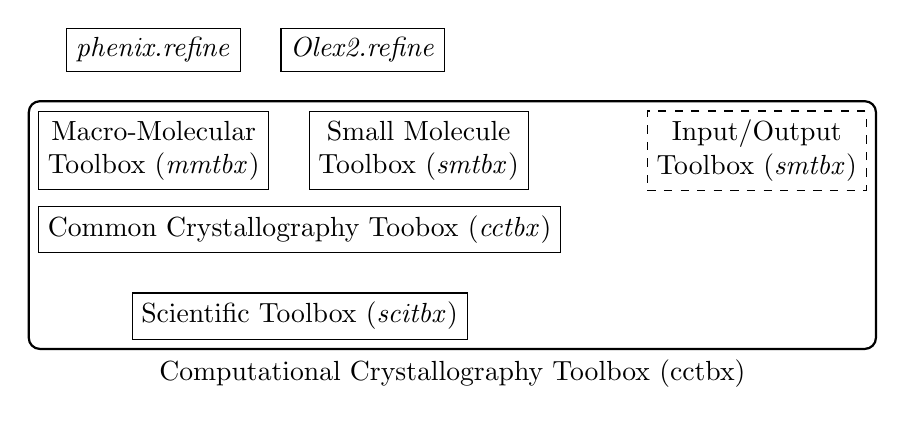
\begin{tikzpicture}[component/.style={draw, shape=rectangle, align=center}, node distance=0.5cm]
\node[component] (phenix) {\phenixrefine};
\node[component, right=of phenix] (olex2) {\Olexrefine};
\node[component, below=of phenix] (mmtbx) {Macro-Molecular \\ Toolbox (\mmtbx)};
\node[component, right=of mmtbx] (smtbx) {Small Molecule \\ Toolbox (\smtbx)};
\node[component, right=1.5 cm of smtbx, style={dashed}] (iotbx) {Input/Output \\ Toolbox (\smtbx)};
\node[component, below=of mmtbx.south west, anchor=west] (cctbx) {Common Crystallography Toobox (\cctbx)};
\node[component, below=of cctbx] (scitbx) {Scientific Toolbox (\scitbx)};
\only<2>{\node[style={draw, rounded corners, thick}, fit={(mmtbx.north west) (iotbx.north east) (scitbx.south)},
        label=below:Computational Crystallography Toolbox (cctbx)] {};}
\end{tikzpicture}
\end{figure}
In Python:
\begin{minted}{python}
from cctbx import sgtbx
\end{minted}
\end{frame}

\begin{frame}[fragile]
\frametitle{Downloads}
\begin{itemize}
\item This tutorial: slides, code and data\\\url{https://github.com/luc-j-bourhis/rovinj-2015-cctbx-tutorial}\item Source and binary packages: \url{http://cci.lbl.gov/cctbx_build/} \\
      Not very up-to-date anymore but it will do for this tutorial!
      \begin{itemize}
      \item Linux: choose CentOS 6.2 (64-bit) even if you don't wear a red hat\\
            \verb!source cctbx_build/setpaths.sh!
      \item Windows 7 (64-bit) or Windows XP (32-bit)\\
            \verb!cctbx_build/setpaths.bat!
      \item \verb!cctbx.python my_script.py!
      \end{itemize}
\item Source code repository (version control): 
\begin{itemize} 
\item Currently hosted on Sourceforge
\item Plans to move to Github soon-ish
\end{itemize}
\end{itemize}
\end{frame}

\begin{frame}[fragile]
\frametitle{Modules}
From the foundations to the roofs:
\begin{itemize}
\item Python $\leftrightarrow$ C++ bridge
\begin{itemize}
\item Python is slow but convenient
\item C++ is fast but cumbersome
\item Boost.Python is a bridge between them and boost\_adaptbx rules it
\end{itemize}
\item scitbx: mathematics, non-crystallographic physics (rigid body)
\begin{itemize}
\item n-dimensional arrays, bridge with NumPy
\item linear algebra, special functions, non-linear least-squares
\end{itemize}
\item cctbx: common crystallography
\begin{itemize}
\item structure factors computation, and their derivatives
\item space group toolbox
\item Fourier transforms
\end{itemize}
\item smtbx: constraints
\begin{itemize}
\item structure factors computation and derivatives
\end{itemize}
\end{itemize}
\end{frame}

\begin{frame}[fragile]
\frametitle{Modules}
Based on cctbx:
\begin{itemize}
\item rstbx: indexing and integration of diffraction images
\item xfel: X-ray free-electron lasers
\item crys3d, gltbx: tools to write GUI displaying 3D objects (structures, Fourier maps)
\begin{itemize}
\item $\longrightarrow$ Phenix
\end{itemize}
\end{itemize}
\end{frame}

\begin{frame}[fragile]
\frametitle{scitbx.matrix}
Matrices in pure Python:
\begin{minted}{python}
>>> from scitbx.matrix import rec, col
>>> A = rec(elems=(-1,0,0, 0,-1,0, 0,0,-1), n=(3,3))
>>> b = col((3,4,5))
>>> C = A * b
>>> print C
matrix.rec(elems=(-3, -4, -5), n=(3,1))
>>> abs(C)
7.0710678118654755
\end{minted}
Matrix written by row: $\begin{bmatrix} -1 & 0 & 0 \\ 0 & -1 & 0 \\ 0 & 0 & -1 \end{bmatrix}$
Use only for few operations on small matrices.
\end{frame}

\begin{frame}[fragile]
\frametitle{scitbx.matrix}
Particularly useful in crystallography
\begin{minted}{python}
>>> from scitbx.matrix import col, row, rt
>>> rt(((-1,0,0, 0,-1,0, 0,0,-1),
       (7,8,9)))*col((3,4,5))
matrix.rec(elems=(4, 4, 4), n=(3,1))
>>> dihedral_angle([(-1,-1,1), (0,0,0), 
                    (1,0,0), (1,1,1)], deg=True)
-90.0
\end{minted}
Used a lot.
\end{frame}

\begin{frame}[fragile]
\frametitle{And now, ladies and gentlement, the main feature!}

Let's triple the unit cell of a structure.

Why, oh, why?

Phase transition: unit cell before the transition $(a, b, c, 90, 90, 90)$, and after $(3a, b, 3c, 90, 90, 90)$.

To compare the two structures, it is useful to put the first one in a tripled unit cell, keeping the same symmetries.


\end{frame}

\end{document}
